% !TEX root= ../main.tex
\section{Inconsistencies in graph theories}
\label{sec:Inconsistencies in graph theories}
In this section, we will prove the existence of non-binary-derivable inconsistencies from graphs.
We will first prove a lemma, then apply this lemma to an extended version of the graph from Figure~\ref{fig:double_open_door} to show that its inconsistency is not binary-derivable.

Let $G$ be a digraph with a source vertex (a vertex with no predecessors) $x$.
Let $A$ and $B$ be two disjoint subgraphs of $G$ such that $N(A) \subseteq A$ and $N(B) \subseteq B$ and such that $N^-(A) \setminus A = N^-(B) \setminus B = \{ x\}$.
In words, nothing points out of $A$ and $B$ and only $x$ points in.
Note that $x$ might have additional successors.\par
\begin{figure}[!h]
  \centering
  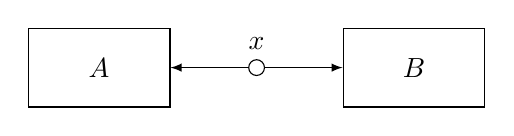
\begin{tikzpicture}
    [
    point/.style={circle,draw,inner sep=0pt,minimum size=2mm},
    collection/.style={rectangle,draw,inner sep=0pt,minimum height=10mm, minimum width= 18mm}
    ]
    \node (x) at (2,0) [point, label=above:$x$] {};
    \node (A) at (0,0) [collection] {$A$};
    \node (B) at (4,0) [collection] {$B$};
    \draw [-latex] (x) to (A);
    \draw [-latex] (x) to (B);
  \end{tikzpicture}
  \caption{Graph $G$}
  \label{fig:components_link}
\end{figure}
A couple of observations can be made from the above construction:
\begin{itemize}
  \item The vertex $x$ only appears in 1 OR-clause, since it is a source vertex.
  This is also the only OR-clause containing a vertex from both $A$ and $B$.
  We will call this OR-clause $X$ and formally define it as $N(x) \cup \{ x\}$.
  \item For any vertex $p$ in $A$ we have that $p$ only appears in axiomatic NAND-clauses together with either $t$ or other vertices in $A$.
  The same obviously holds for any vertex in $B$.
\end{itemize}
Based on graph $G$ from Figure~\ref{fig:components_link} we now introduce the following lemma:
\begin{lemma}
  Given two vertice $a \in A$ and $b \in B$; if $\ol{ab}$ is provable in Neg, then the proof must contain the OR-clause $X$.
  \label{thm:or_clause_lemma}
\end{lemma}
The lemma will be proven by inducing over the length of the proof of $\ol{ab}$.
\begin{proof}
  In the base case, the proof length is 1, so $\ol{ab}$ is the direct conclusion from a premise with axioms only.
  \begin{figure}[!h]
    \centering
    \begin{prooftree*}
      \Hypo{\ol{ap}}
      \Hypo{\ol{bq}}
      \Hypo{\dots}
      \Infer[right label=$X$]3{\ol{ab}}
    \end{prooftree*}
    \caption{}
    \label{fig:ab_proof_bc}
  \end{figure}
  The premise must contain one axiom on the form $\ol{ap}$ and one on the form $\ol{bq}$.
  If either $p = x$ or $q = x$, then the OR-clause used in the proof step must be $X$, being the only OR-clause containing $x$.
  On the other hand, if neither $p$ nor $q$ equals $x$, then $p \in A$ and $q \in B$.
  Since $X$ is the only OR-clause containing vertices from both $A$ and $B$, $X$ is again our only choice.
  A proof of $\ol{ab}$ of length 1 must hence use the OR-clause $X$.

  For the inductive step, we assume that for any proof of length $k-1$; if it concludes with a NAND-clause $\ol{pq}$ such that $p$ and $q$ are from differen components, then it must use the OR-clause $X$ somewhere.
  This assumption makes us able to prove the inductive step in almost exactly the same way as with the base case.

  Suppose there is a proof of length $k$ concluding with $\ol{ab}$.
  Its immediate premise must contain one NAND-clause on the form $\ol{ap}$ and one on the form $\ol{bq}$.
  Again, if either $p=x$ or $q=x$, or if $p \in A$ and $q \in B$, the OR-clause $X$ must be used, by the same argument as in the base case.
  This leaves us with the case where either $p \not\in A$ or $q \not\in B$.
  Our induction hypothesis gives us that the proof of either of those contains $X$ somewhere.

  A proof of length $k$ concluding with $\ol{ab}$ must therefore use the OR-clause $X$, so we can conclude that \textit{any} proof of $\ol{ab}$ must contain $X$.
\end{proof}

Consider now the following graph, containing 3 copies of our graph from Figure~\ref{fig:double_open_door}, one northern (N), one western (W) and one eastern (E).\par
\begin{figure}[!h]
  \centering
  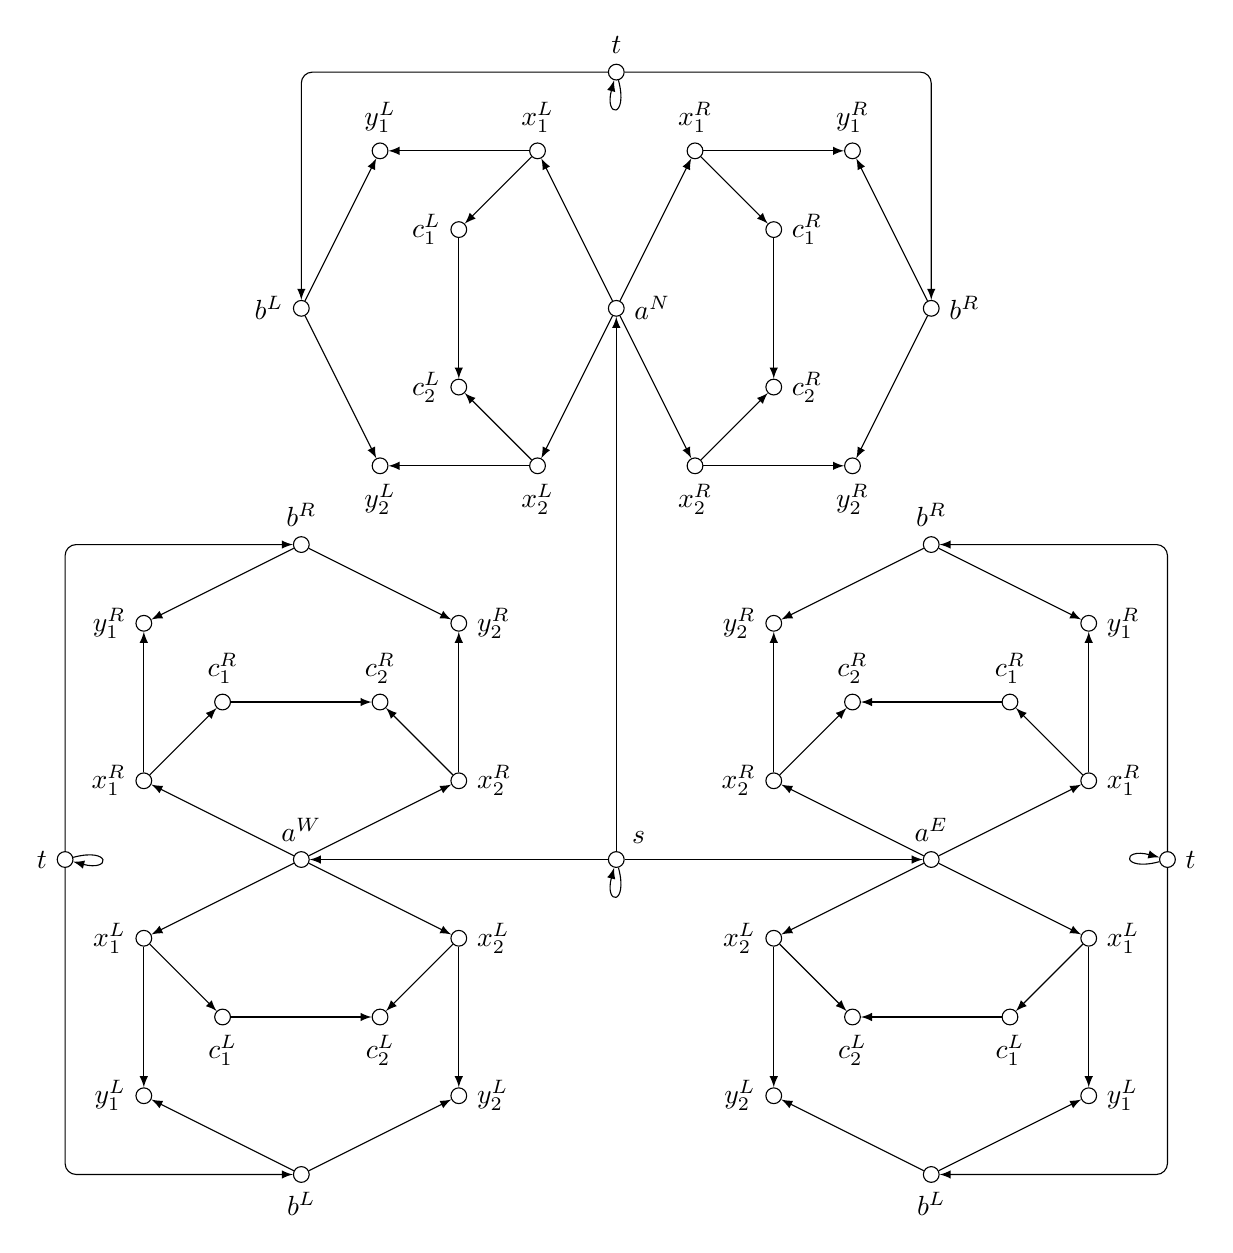
\begin{tikzpicture}
    [
    point/.style={circle,draw,inner sep=0pt,minimum size=2mm}
    ]
    \node (t) at (7,14) [point,label=above:$t$] {};
    \node (a) at (7,11) [point,label=right:$a^N$] {};
    \node (lx1) at (6,13) [point,label=above:$x^L_1$] {};
    \node (lx2) at (6,9) [point,label=below:$x^L_2$] {};
    \node (lb) at (3,11) [point,label=left:$b^L$] {};
    \node (ly1) at (4,13) [point,label=above:$y^L_1$] {};
    \node (ly2) at (4,9) [point,label=below:$y^L_2$] {};
    \node (lc1) at (5,12) [point,label=left:$c^L_1$] {};
    \node (lc2) at (5,10) [point,label=left:$c^L_2$] {};
    \draw [-latex] (a) to (lx1);
    \draw [-latex] (a) to (lx2);
    \draw [-latex] (lb) to (ly1);
    \draw [-latex] (lb) to (ly2);
    \draw [-latex] (lx1) to (ly1);
    \draw [-latex] (lx1) to (lc1);
    \draw [-latex] (lx2) to (ly2);
    \draw [-latex] (lx2) to (lc2);
    \draw [-latex] (lc1) to (lc2);
    \node (rx1) at (8,13) [point,label=above:$x^R_1$] {};
    \node (rx2) at (8,9) [point,label=below:$x^R_2$] {};
    \node (rb) at (11,11) [point,label=right:$b^R$] {};
    \node (ry1) at (10,13) [point,label=above:$y^R_1$] {};
    \node (ry2) at (10,9) [point,label=below:$y^R_2$] {};
    \node (rc1) at (9,12) [point,label=right:$c^R_1$] {};
    \node (rc2) at (9,10) [point,label=right:$c^R_2$] {};
    \draw [-latex] (a) to (rx1);
    \draw [-latex] (a) to (rx2);
    \draw [-latex] (rb) to (ry1);
    \draw [-latex] (rb) to (ry2);
    \draw [-latex] (rx1) to (ry1);
    \draw [-latex] (rx1) to (rc1);
    \draw [-latex] (rx2) to (ry2);
    \draw [-latex] (rx2) to (rc2);
    \draw [-latex] (rc1) to (rc2);
    \draw [-latex, rounded corners] (t) -| (lb);
    \draw [-latex, rounded corners] (t) -| (rb);
    \draw [-latex, loop below] (t) to (t);

    \node (wt) at (0,4) [point,label=left:$t$] {};
    \node (wa) at (3,4) [point,label=above:$a^W$] {};
    \node (wlx1) at (1,3) [point,label=left:$x^L_1$] {};
    \node (wlx2) at (5,3) [point,label=right:$x^L_2$] {};
    \node (wlb) at (3,0) [point,label=below:$b^L$] {};
    \node (wly1) at (1,1) [point,label=left:$y^L_1$] {};
    \node (wly2) at (5,1) [point,label=right:$y^L_2$] {};
    \node (wlc1) at (2,2) [point,label=below:$c^L_1$] {};
    \node (wlc2) at (4,2) [point,label=below:$c^L_2$] {};
    \draw [-latex] (wa) to (wlx1);
    \draw [-latex] (wa) to (wlx2);
    \draw [-latex] (wlb) to (wly1);
    \draw [-latex] (wlb) to (wly2);
    \draw [-latex] (wlx1) to (wly1);
    \draw [-latex] (wlx1) to (wlc1);
    \draw [-latex] (wlx2) to (wly2);
    \draw [-latex] (wlx2) to (wlc2);
    \draw [-latex] (wlc1) to (wlc2);
    \node (wrx1) at (1,5) [point,label=left:$x^R_1$] {};
    \node (wrx2) at (5,5) [point,label=right:$x^R_2$] {};
    \node (wrb) at (3,8) [point,label=above:$b^R$] {};
    \node (wry1) at (1,7) [point,label=left:$y^R_1$] {};
    \node (wry2) at (5,7) [point,label=right:$y^R_2$] {};
    \node (wrc1) at (2,6) [point,label=above:$c^R_1$] {};
    \node (wrc2) at (4,6) [point,label=above:$c^R_2$] {};
    \draw [-latex] (wa) to (wrx1);
    \draw [-latex] (wa) to (wrx2);
    \draw [-latex] (wrb) to (wry1);
    \draw [-latex] (wrb) to (wry2);
    \draw [-latex] (wrx1) to (wry1);
    \draw [-latex] (wrx1) to (wrc1);
    \draw [-latex] (wrx2) to (wry2);
    \draw [-latex] (wrx2) to (wrc2);
    \draw [-latex] (wrc1) to (wrc2);
    \draw [-latex, rounded corners] (wt) |- (wlb);
    \draw [-latex, rounded corners] (wt) |- (wrb);
    \draw [-latex, loop right] (wt) to (wt);

    \node (et) at (14,4) [point,label=right:$t$] {};
    \node (ea) at (11,4) [point,label=above:$a^E$] {};
    \node (elx1) at (13,3) [point,label=right:$x^L_1$] {};
    \node (elx2) at (9,3) [point,label=left:$x^L_2$] {};
    \node (elb) at (11,0) [point,label=below:$b^L$] {};
    \node (ely1) at (13,1) [point,label=right:$y^L_1$] {};
    \node (ely2) at (9,1) [point,label=left:$y^L_2$] {};
    \node (elc1) at (12,2) [point,label=below:$c^L_1$] {};
    \node (elc2) at (10,2) [point,label=below:$c^L_2$] {};
    \draw [-latex] (ea) to (elx1);
    \draw [-latex] (ea) to (elx2);
    \draw [-latex] (elb) to (ely1);
    \draw [-latex] (elb) to (ely2);
    \draw [-latex] (elx1) to (ely1);
    \draw [-latex] (elx1) to (elc1);
    \draw [-latex] (elx2) to (ely2);
    \draw [-latex] (elx2) to (elc2);
    \draw [-latex] (elc1) to (elc2);
    \node (erx1) at (13,5) [point,label=right:$x^R_1$] {};
    \node (erx2) at (9,5) [point,label=left:$x^R_2$] {};
    \node (erb) at (11,8) [point,label=above:$b^R$] {};
    \node (ery1) at (13,7) [point,label=right:$y^R_1$] {};
    \node (ery2) at (9,7) [point,label=left:$y^R_2$] {};
    \node (erc1) at (12,6) [point,label=above:$c^R_1$] {};
    \node (erc2) at (10,6) [point,label=above:$c^R_2$] {};
    \draw [-latex] (ea) to (erx1);
    \draw [-latex] (ea) to (erx2);
    \draw [-latex] (erb) to (ery1);
    \draw [-latex] (erb) to (ery2);
    \draw [-latex] (erx1) to (ery1);
    \draw [-latex] (erx1) to (erc1);
    \draw [-latex] (erx2) to (ery2);
    \draw [-latex] (erx2) to (erc2);
    \draw [-latex] (erc1) to (erc2);
    \draw [-latex, rounded corners] (et) |- (elb);
    \draw [-latex, rounded corners] (et) |- (erb);
    \draw [-latex, loop left] (et) to (et);

    \node (s) at (7,4) [point,label=above right:$s$] {};
    \draw [-latex] (s) to (a);
    \draw [-latex] (s) to (wa);
    \draw [-latex] (s) to (ea);
    \draw [-latex,loop below] (s) to (s);
  \end{tikzpicture}
  \caption{}
  \label{fig:triple_double_open_door}
\end{figure}
The proof of $\ol{a}$ from Figure~\ref{fig:unary_nand_proof} can be applied to each component in the above graph, giving us the provability of $\ol{a^N}$, $\ol{a^W}$ and $\ol{a^E}$.
From here, the inconsistency proof is trivial:\par
\begin{figure}[!h]
  \centering
  \begin{prooftree*}
    \Hypo{\ol{s}}
    \Hypo{\dots}
    \Infer[]1{\ol{a^N}}
    \Hypo{\dots}
    \Infer[]1{\ol{a^W}}
    \Hypo{\dots}
    \Infer[]1{\ol{a^W}}
    \Infer[right label=$sa^Na^Wa^E$]4{\varnothing}
  \end{prooftree*}
  \caption{}
  \label{fig:triple_double_open_door_proof}
\end{figure}
The above graph is thus provably inconsistent.
We will now show that the inconsistency is non-binary-derivable.

The first thing to notice is that if one removes the loop on vertex $s$, the graph is no longer inconsistent.
This tells us that the NAND-clause $\ol{s}$ must be in any inconsistency proof.
If that was not the case, we would be able to prove $\varnothing$ on a graph that was not inconsistent, violating the fact that Neg is sound.

Having that any inconsistency proof contains $\ol{s}$ immediately gives us that any inconsistency proof contains the OR-clause $sa^Na^Wa^E$, since this is the only OR-clause containing $s$.
We thus have the following situation somewhere in the proof, where the sets of vertices $P,Q,R$ might be empty:\par
\begin{figure}[!h]
  \centering
  \begin{prooftree*}
    \Hypo{\ol{s}}
    \Hypo{\dots}
    \Infer[]1{\ol{a^NP}}
    \Hypo{\dots}
    \Infer[]1{\ol{a^WQ}}
    \Hypo{\dots}
    \Infer[]1{\ol{a^WR}}
    \Infer[right label=$sa^Na^Wa^E$]4{\ol{P \cup Q \cup R}}
  \end{prooftree*}
  \caption{}
  \label{fig:triple_double_proof_step}
\end{figure}
The OR-clause in question might obviously appear several places in the proof, but let us assume that this is its \textit{first} appearance, i.e. none of the NAND-clauses in the premise are proven using the OR-clause $sa^Na^Wa^E$.

First of all, neither of the sets $P,Q,R$ can contain more than 1 element, since that would make the NAND-clauses non-binary.
For the same reason can their union never contain more than two elements, since that would make the concluding NAND-clause non-binary.
One of them must thus either be empty, or some of them must contain the same element.

Let us first assume that neither of $P,Q,R$ are empty.
This implies that at least two of them contain the same element.
We will now apply Lemma~\ref{thm:or_clause_lemma} to show that this is not possible.

Observe that our graph consists of three isolated components, $N$, $W$ and $E$, only connected by the vertex $s$ having a vertex from each component in its neighborhood.
Let, without any loss of generality, $P$ and $Q$ be the two sets with the same element, i.e., $P = Q = \{p\}$.
That gives us the two NAND-clauses $\ol{a^Np}$ and $\ol{a^Wp}$.
Since our three components are mutually disjoint, at least one of the above NAND-clauses must contain vertices from two different components.\todo{one of them can be $s$; should be mentioned.}
Lemma~\ref{thm:or_clause_lemma} gives us that the proof of that NAND-clause therefore must contain the OR-clause $sa^Na^Wa^E$, which contradicts our assumption of it being used for the first time in Figure~\ref{fig:triple_double_proof_step}.
Therefore, none of the three $a$-clauses in the premise can contain the same element, leaving us with the case where one of them is unary, i.e. either $P$, $Q$ or $R$ is empty.

Now, we know that both $\ol{a^N}$, $\ol{a^W}$ and $\ol{a^E}$ are provable, but the only proof we have seen has been non-binary, using the proofs of $\ol{ab}$ as subproofs.
The last section showed that $\ol{a}$ was not provable if one was only to use the vertices from within its own component.
So if one of the $a$-clauses in the premise in Figure~\ref{fig:triple_double_proof_step} is unary, then it has to have been proved using either $s$ or vertices from other components.
In both cases, we get that such a proof must contain the OR-clause $sa^Na^Wa^E$ somewhere, again contradicting our assumption.

All in all, this gives us that if the proof is binary up until this rule application, the concluding NAND-clause cannot be binary.
Since the rule application has to be present in the inconsistency proof, the proof therefore has to contain a non-binary NAND-clause, indeed making the inconsistency non-binary-derivable.
